\documentclass[xcolor=pdftex,dvipsnames,table]{beamer}
\usepackage{beamerthemesplit}
\usetheme{Copenhagen}
\useoutertheme{shadow}
\useinnertheme{rounded}
\usepackage{color}
\usepackage{graphicx}
\usepackage{fancybox}


\title{Website Changes and User Behavior}
\subtitle{Using Panjiva Data to Examine Code Changes}
\author{John J. Wang}
\date{\today}
\institute{14.27 Final Presentation}

\begin{document}

\frame{\titlepage}

\section[Outline]{}
\frame{\tableofcontents}

\section[Introduction]{Introduction}

\subsection[Silicon Valley]{Silicon Valley Mindset}

\frame{
    \frametitle{The Silicon Valley Mindset}
    \begin{itemize}
        \item "Move fast and break things." -- Facebook
        \item "The only constant is change itself." -- Heraclitus
        \item "Pick a movement, pick a revolution, and join it." -- Jack Dorsey
    \end{itemize}
}

\subsection{What We Know}
\frame
{
    \frametitle{Background and Previous Research}
    \begin{itemize}
        \item Levitt and Fryer 2004
        \item Neal 2005
        \item Brooks Gunn et al 1993, 1996, 2000
    \end{itemize}
}

\subsection{Questions to Ask}
\frame
{
    \frametitle{Lingering Questions}
    \begin{itemize}
        \item Do users tend to respond favorably to website changes?
        \item How do users react to different types of change?
        \item How do different characteristics of users affect their reactions to change?
    \end{itemize}
    \end{block}
}

\subsection{Panjiva Dataset}

\frame
{
    \frametitle{Panjiva, Inc.}
    \begin{itemize}
        \item \url{http://www.panjiva.com}
        \item Acts as a medium for buyers and suppliers of manufactured goods
        \item Parses government import and export data for unbiased shipment information on suppliers
        \item Example: Home Depot finding a wrench factory
    \end{itemize}
}

\frame
{
    \frametitle{Summary Statistics}
    \begin{table}[h!]
    \centering
    \caption{Panjiva Overview}
    \begin{tabular}{l || l}
    \hline
    Total Users & 121,653 \\
    Subscribing Users & 2,985 \\
    Monthly Site Visits & 903,426 \\
    Monthly Unique Visitors & 762,723 \\
    Average Pages per Visit & 1.99 \\
    Average Visit Duration & 1 min 18 sec \\
    \hline
    \end{tabular}
    \label{table:panjiva-overview}
    \end{table}
}

\frame
{
    \frametitle[Event and Activity Logs}
    \begin{itemize}
        \item Event Logs contain records of all user actions $\sim 124$ million records
        \item Activity Logs contain records of actions of users who are registered with Panjiva $\sim 13$ million records
    \end{itemize}
}

\frame
{
    \frametitle{Commit Statistics}
    \begin{table}[h!]
    \centering
    \caption{Overall Commit Statistics - 11/25/2012}
    \begin{tabular}{l || l }
    \hline
    Active Days (at least 1 commit) & 1,983 \\
    Total Current Files & 20,901 \\
    Total Lines of Code & 1,313,235 \\
    Total Lines of Code Added & 3,989,295 \\
    Total Lines of Code Removed & 2,676,060 \\
    Total Commits & 29,924 \\
    Total Authors/Developers & 33 \\
    \hline
    \end{tabular}
    \label{table:commit-stats}
    \end{table}
} 

\frame
{
    \frametitle{Commit Frequency by Time of Day}
    \begin{figure}[h!]
    \centering
    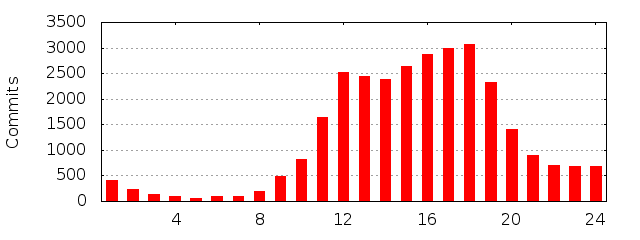
\includegraphics[width=4in]{pictures/commit-hours.png}
    \caption{Number of Commits by Hour of the Day}
    \label{fig:commit-hours}
    \end{figure}

}

\section{Macro-Level Results}

\subsection{Daily Effects of Code Changes}

\frame
{
    \frametitle{Specification}
    \begin{eqnarray}
    y^i_{t} = c_0 + \vec{\gamma}^T \vec{M}_t + \vec{\beta}^T \vec{\chi}_t + \epsilon_t
    \end{eqnarray}

    \begin{itemize}
        \item $t$ indexes day
        \item $y^i_t$ corresponds to $i$th metric of user activity on day $t$
        \item $\vec{M}_t$ corresponds to a vector of covariates that represent changes in the code
        \item $\vec{\chi}_t$ is a vector of controls
    \end{itemize}
}   

\frame
{
    \frametitle{Effect of Commits on User Activity}
    \begin{table}[h!]
    \footnotesize
    \centering
    {
        \def\sym#1{\ifmmode^{#1}\else\(^{#1}\)\fi}
        \begin{tabular}{l*{2}{c}}
        \hline\hline
            &\multicolumn{1}{c}{(1)}&\multicolumn{1}{c}{(2)}\\
            &\multicolumn{1}{c}{activitylogcount}&\multicolumn{1}{c}{eventlogcount}\\
            \hline
            fileschanged&     -5530.7         &    -60589.4\sym{*}  \\
 percentile           &     (-1.91)         &     (-2.26)   \\
            [1em]
            insertions&      4868.8\sym{*}  &     47053.7\sym{*} \\
percentile
    &      (2.12)         &      (2.22)         \\
        [1em]
        deletions&      2778.9         &     29970.6    \\
        percentile&      (1.29)         &      (1.50)   \\
        [1em]
        weekend     &    -14708.0\sym{***}&    -79769.8\sym{***}\\
        &    (-16.48)         &     (-9.65)      \\
        [1em]
        \_cons      &     22396.6\sym{***}&    224482.8\sym{***}\\
        &     (25.05)         &     (27.12)      \\
        \hline
        \(N\)       &         474         &         475     \\
        \hline\hline
        \multicolumn{3}{l}{\footnotesize \textit{t} statistics in parentheses}\\
        \multicolumn{3}{l}{\footnotesize \sym{*} \(p<0.05\), \sym{**} \(p<0.01\), \sym{***} \(p<0.001\)}\\
        \end{tabular}
    }
    \end{table}
}

\frame
{
    \frametitle{Effect of Commits on User Activity}
    \begin{table}[h!]
    \footnotesize
    \centering
    {
        \def\sym#1{\ifmmode^{#1}\else\(^{#1}\)\fi}
        \begin{tabular}{l*{2}{c}}
        \hline\hline
            &\multicolumn{1}{c}{(1)}&\multicolumn{1}{c}{(2)}\\
            &\multicolumn{1}{c}{avguseractivity}&\multicolumn{1}{c}{avguserevents}\\
            \hline
            fileschanged&     -10.40\sym{*}         &    -148.6  \\
 percentile           &     (-2.01)         &     (-1.52)   \\
            [1em]
            insertions&      2.817  &     79.92 \\
percentile
    &      (0.69)         &      (1.03)         \\
        [1em]
        deletions&      4.670        &    49.47    \\
        percentile&      (1.21)         &      (0.68)   \\
        [1em]
        weekend     &    -0.297&    257.0\sym{***}\\
        &    (-0.19)         &     (8.49)      \\
        [1em]
        \_cons      &     25.00\sym{***}&    340.6\sym{***}\\
        &     (15.58)         &     (11.24)      \\
        \hline
        \(N\)       &         474         &         475     \\
        \hline\hline
        \multicolumn{3}{l}{\footnotesize \textit{t} statistics in parentheses}\\
        \multicolumn{3}{l}{\footnotesize \sym{*} \(p<0.05\), \sym{**} \(p<0.01\), \sym{***} \(p<0.001\)}\\
        \end{tabular}
    }
    \end{table}
}

\subsection{Lagged Effects of Code Changes}

\frame
{
    \frametitle{Specification}
    \begin{eqnarray}
    y^i_{tx} = c_0 + \gamma M_{t} + \beta weekend_{t} + \epsilon_t
    \end{eqnarray}

    \begin{itemize}
        \item Lag variable $x \in [1,30]$. 
        \item Examines how commits on day $t$ affect user behavior in time $t + x$. 
    \end{itemize}

}

\frame
{
    \frametitle{Average Activity Logs Per Distinct User}
    \begin{figure}[h!]
    \centering
    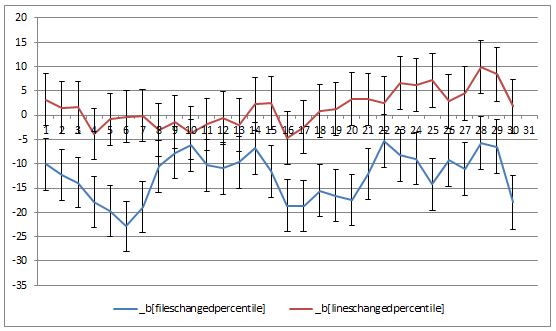
\includegraphics[width=4in]{pictures/avg_activities_time_coefficients.png}
    \label{fig:avg-activities-time-coefficients}
    \caption{$\gamma$ Coefficients with Varying Lags, Regressed on Average Activity Logs per User}
    \end{figure}
}

\frame
{
    \frametitle{Average Event Logs Per Distinct User}
    \begin{figure}[h!]
    \centering
    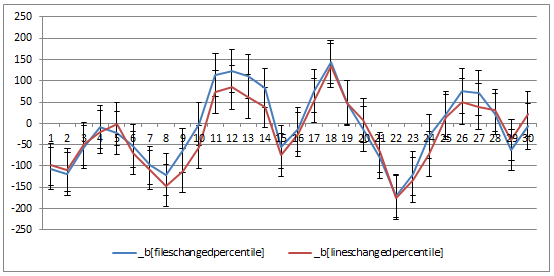
\includegraphics[width=4in]{pictures/avg_events_time_coefficients.png}
    \caption{$\gamma$ Coefficients with Varying Lags, Regressed on Average Event Logs per User}
    \label{fig:avg-events-time-coefficients}
    \end{figure}
}

\frame
{
    \frametitle{Insertions and Deletions}
    \begin{figure}[h!]
    \centering
    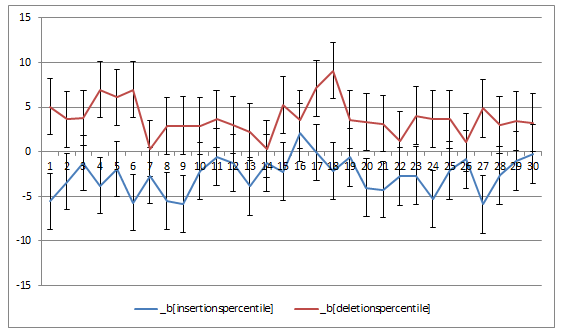
\includegraphics[width=3.7in]{pictures/commit_percentiles_time_coefficients.png}
    \label{fig:insertions-deletions-time-coefficients}
    \caption{$\gamma_0$ and $\gamma_1$ Coefficients with Varying Lags. Regressed on Average Activity Logs per User}
    \centering
    \end{figure}
}

\section{Micro-Level Results}

\frame
{
    \frametitle{Problems with Macro-Level Data}
    \begin{itemize}
    \item Nothing more than correlations
    \item Possibly complex, unknown mechanisms for how results come about
    \end{itemize}
}

\frame
{
    \frametitle{The Case for Micro-Level Data}
    \begin{itemize}
    \item Panjiva has data on the page and time that any action was performed.
    \item Code changes (commits) can be thought of as exogeneous shocks.
        \subitem Changes are unannounced
        \subitem Only extremely large changes are announced on blog (less than 1\% of Panjiva's total pageviews come from blog).
    \end{itemize}
}

\subsection{Search Controller}

\frame
{
    \frametitle{Search Controller}
    \begin{figure}
    \centering
    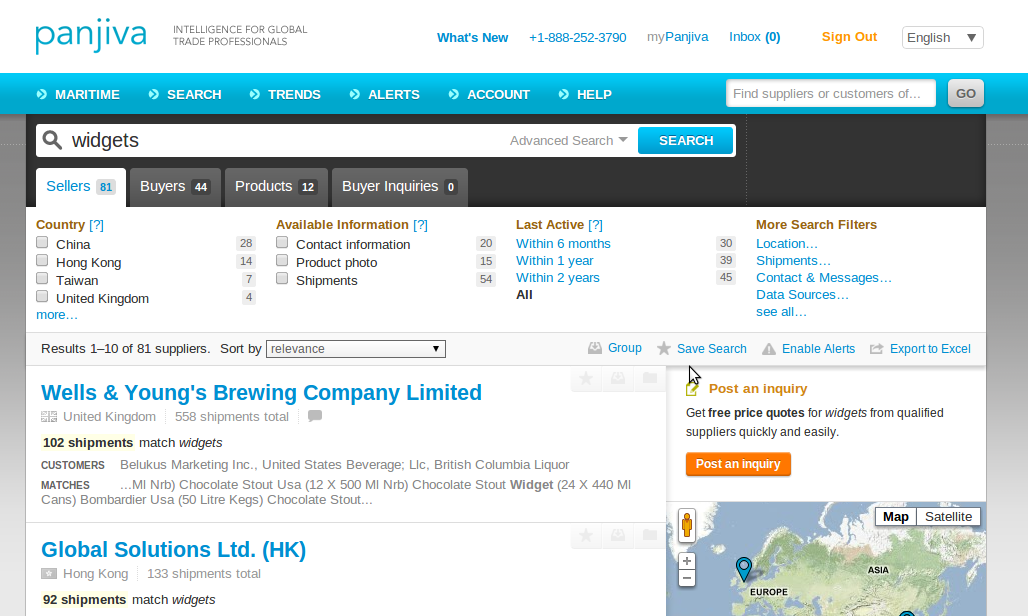
\includegraphics[width=3in]{pictures/search_page.png}
    \caption{The Search Page, Panjiva's most trafficked page, provides functionality for finding suppliers, buyers, products, and buyer inquiries.}
    \end{figure}
}

\frame
{
    \frametitle{Specification}
    \begin{eqnarray}
    num\_views\_day\_after_{it} = c_0 + \beta_0 \mu_{it} + \beta_1 hour\_dummies_{it} + \epsilon_{it}
    \end{eqnarray}

    \begin{itemize}
        \item $i$ indexes the $i$th commit and $t$ is the $t$th view in 4 day window surround the $i$th commit.
        \item $\mu_{it}$ is either $after\_commit$ or $time\_from\_event$. 
    \end{itemize}
}

\frame
{
    \frametitle{Visualization of Variables}

}

\frame
{
    \frametitle{Search Regression Results}
    \centering
    {
        \def\sym#1{\ifmmode^{#1}\else\(^{#1}\)\fi}
        \begin{tabular}{l*{4}{c}}
        \hline\hline
            & \multicolumn{4}{l}{Independent Variable: num\_views\_day\_later} \\
            &\multicolumn{1}{c}{(1)}&\multicolumn{1}{c}{(2)}&\multicolumn{1}{c}{(3)}&\multicolumn{1}{c}{(4)}\\
            \hline
            after\_commit&       5.541\sym{***}&               &       3.378\sym{***}&                     \\
            &     (17.91)         &                     &     (11.20)         &                     \\
            [1em]
            time\_from\_event&                     &   0.0000737\sym{***}&                     &    0.000110\sym{***}\\
            &                    &     (43.76)         &                     &     (66.60)         \\
            [1em]
            created\_at\_hour&             No        &           No           &       Yes &      Yes \\
            dummies?&                     &                     &              &            \\
            [1em]
            \_cons      &       156.9\sym{***}&       159.9\sym{***}&       138.3\sym{***}&       139.7\sym{***}\\
            &    (731.32)     &   (1033.47)         &    (127.71)         &    (130.50)         \\
            \hline
            \(N\)       &     2345617       &     2345617         &     2345617         &     2345617         \\
            \hline\hline
            \multicolumn{5}{l}{\footnotesize \textit{t} statistics in parentheses, \sym{*} \(p<0.05\), \sym{**} \(p<0.01\), \sym{***} \(p<0.001\)}\\
            \end{tabular}
        }
}

\end{document}


